\documentclass{beamer}
\usepackage[utf8]{inputenc}
\usepackage[final]{pdfpages}
\usetheme{Goettingen}%Warsaw}
\usecolortheme{lily}
\setbeamertemplate{footline}[page number]
\title[Fast classification]{Efficient dynamic and static environment classification in Occupancy Grid framework}
\author{Jander Nascimento}
\institute{Université Joseph Fourier / INRIA}
\date{\today}
\begin{document}

\begin{frame}
\titlepage
\end{frame}

%\AtBeginSubsection[]
{
  \begin{frame}<beamer>
    \frametitle{Roadmap}
    \tableofcontents%[currentsection,currentsubsection]
  \end{frame}
}

\section{Problem}

	\begin{frame}
		\frametitle{BOF overview}
		\begin{block}{Goal}
			 Provide only moving cells to BOF
		\end{block}
		 
		Constrains
		\begin{itemize}
			\item In a car (platform)
			\item using a laser scanner (sensor)
			\item As fast as possible (online)
		\end{itemize}
		
		Expectation
		\begin{itemize}
			\item Improve the BOF results
			\item Improve the performance (adapting the BOF)
		\end{itemize}

	\end{frame}


\section{Introduction}

	\begin{frame}
		\frametitle{ADAS}
		\begin{exampleblock}{Stands for}	
			Advanced Driver Assistance Systems		
		\end{exampleblock}				
		\begin{block}{Canonical definition}
			Cope with vehicle handling tasks
		\end{block}		
		\begin{block}{Goal}
			\begin{itemize}
			\item Reduce the risk of collisions
			\item Reduce the driver overload
			\item Increase the confort
			\end{itemize}
		\end{block}
		\begin{block}{Definition}
				The process of acquiring knowledge about the environment \cite{iyengar1991autonomous}
		\end{block}
	\end{frame}

\section{Perception process}


	\begin{frame}
		\frametitle{Grouping process in robotics}	
		\begin{exampleblock}{SLAM}		
			\begin{quotation}
... providing the vehicle with a map of static parts of the environment as well as its location in the map \cite{DBLP:journals/inffus/VuBA11}
			\end{quotation}
			\begin{itemize}
			\item Localization
			\item Mapping
			\end{itemize}			
		\end{exampleblock}					
				
		\begin{exampleblock}{DATMO}		
			\begin{quotation}
			... being aware of dynamic entities around, tracking them, and knowing their future position \cite{DBLP:journals/inffus/VuBA11}
			\end{quotation}				
			\begin{itemize}
			\item Moving objects
				\begin{itemize}
				\item Detection
				\item Tracking
				\end{itemize}			
			\end{itemize}			
		\end{exampleblock}						
				
	\end{frame}

%%%%%%%%%%%%%%%%%%%%%%%%%%%%%%%%%%%%%

\section{State of the art}

	\begin{frame}
		\frametitle{State of the art}
		
		\begin{block}{Other static/dynamic classification}
			\begin{itemize}
			\item "Use a Single Camera for Simultaneous Localization And Mapping with  Mobile Object Tracking in dynamic environments" \cite{Migliore_2009_ICRA}
				\begin{itemize}			
				\item EKF for tracking, with two models				
				\end{itemize}		
			\item "Mapping in dynamic environments using stereo vision" \cite{DBLP:conf/ivs/LategahnGHKE11}
				\begin{itemize}
				\item Disparity image to find the contour
				\item Classifier based on SPRT				
				\end{itemize}		
			\item "Grid-based localization and local mapping with moving object detection and tracking" \cite{Vu201158}
				\begin{itemize}			
				\item MHT + IMM			
				\end{itemize}	
			\end{itemize}		
		\end{block}
	\end{frame}

\section{Motion Detection}

	\begin{frame}
		\frametitle{Solution overview}
		\begin{figure}[h]
			\center
			\includegraphics[scale=0.5]{img/fig:problem}
		 \end{figure}
		 
		\begin{block}{Problem}
			 Being able to identify the dynamic parts of the environment
		\end{block}
		 
		\begin{block}{Result}
			High level classification
		\end{block}				 

		\begin{alertblock}{Not our goal}
			solve DATMO and SLAM
		\end{alertblock}
	\end{frame}

\subsection{preprocessing}

	\begin{frame}
		\frametitle{Experimental Platform}
		\begin{figure}[h]
			\center
			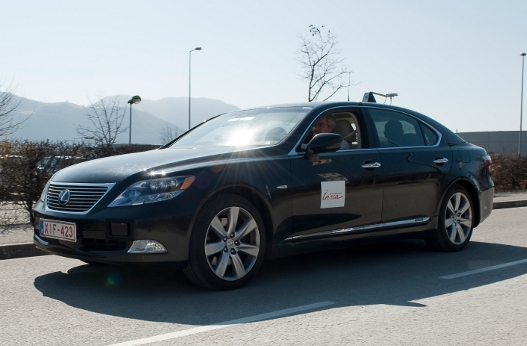
\includegraphics[scale=0.8]{../img/testbed:car}
		  \end{figure}		
		
		  \begin{columns}[t]
		  \begin{column}{5cm}
		  \begin{figure}[h]
			\center
			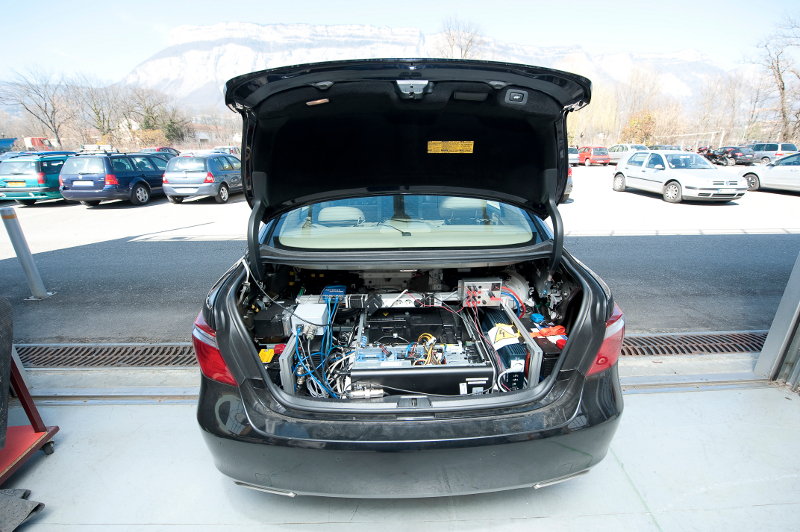
\includegraphics[scale=0.7]{../img/testbed:trunc}
		  \end{figure}
		  \end{column}
		  
		  \begin{column}{5cm}
		  \begin{figure}[h]
			\center
			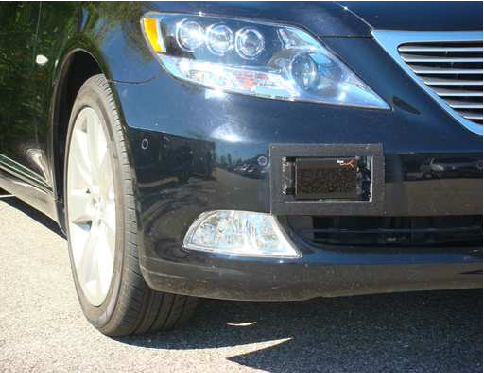
\includegraphics[scale=0.26]{../img/testbed:ibeo}
		  \end{figure}   
		  \end{column}
		 \end{columns}		 
	\end{frame}

	\begin{frame}
		\frametitle{Experimental Platform}
		\begin{figure}[h]
			\center
			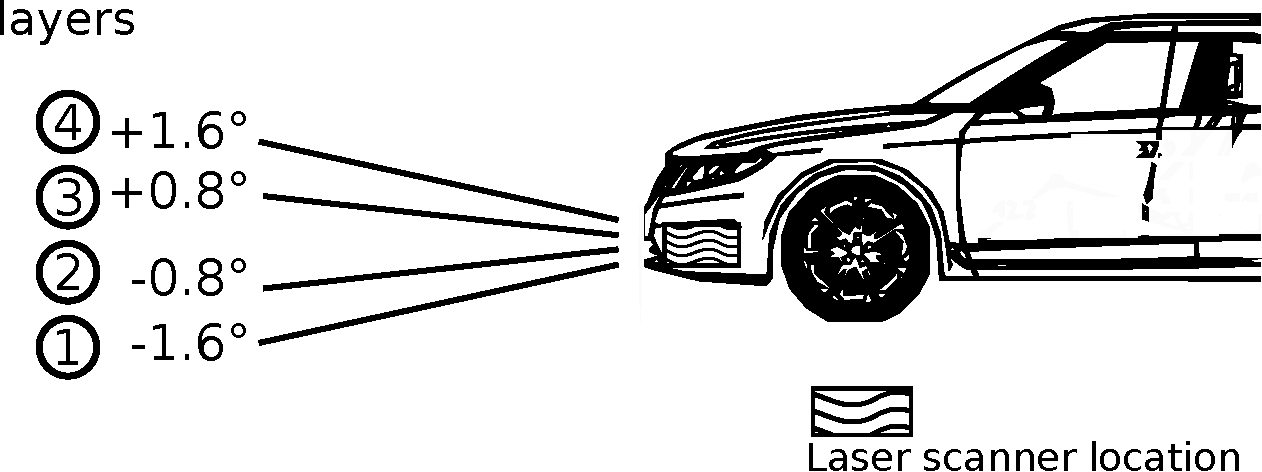
\includegraphics[scale=0.4]{../img/fig:demonstrator:lateral}
		\end{figure}
	\end{frame}

	\begin{frame}
		\frametitle{Experimental Platform}	
		 \begin{columns}[t]
		  \begin{column}{5cm}
		  \begin{figure}[h]
			\center
			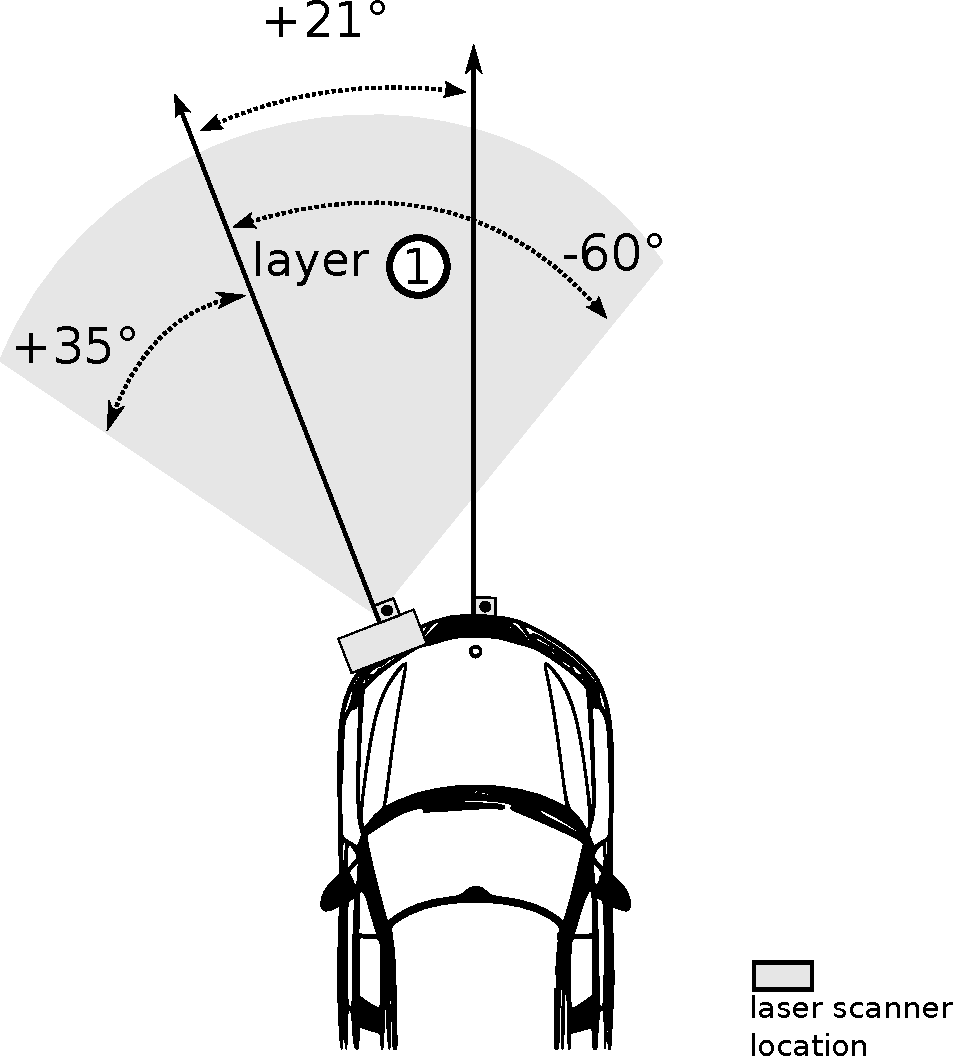
\includegraphics[scale=0.3]{../img/fig:demonstrator:superior}
		  \end{figure}
		  \end{column}
		  
		  \begin{column}{5cm}
		  \begin{figure}[h]
			\center
			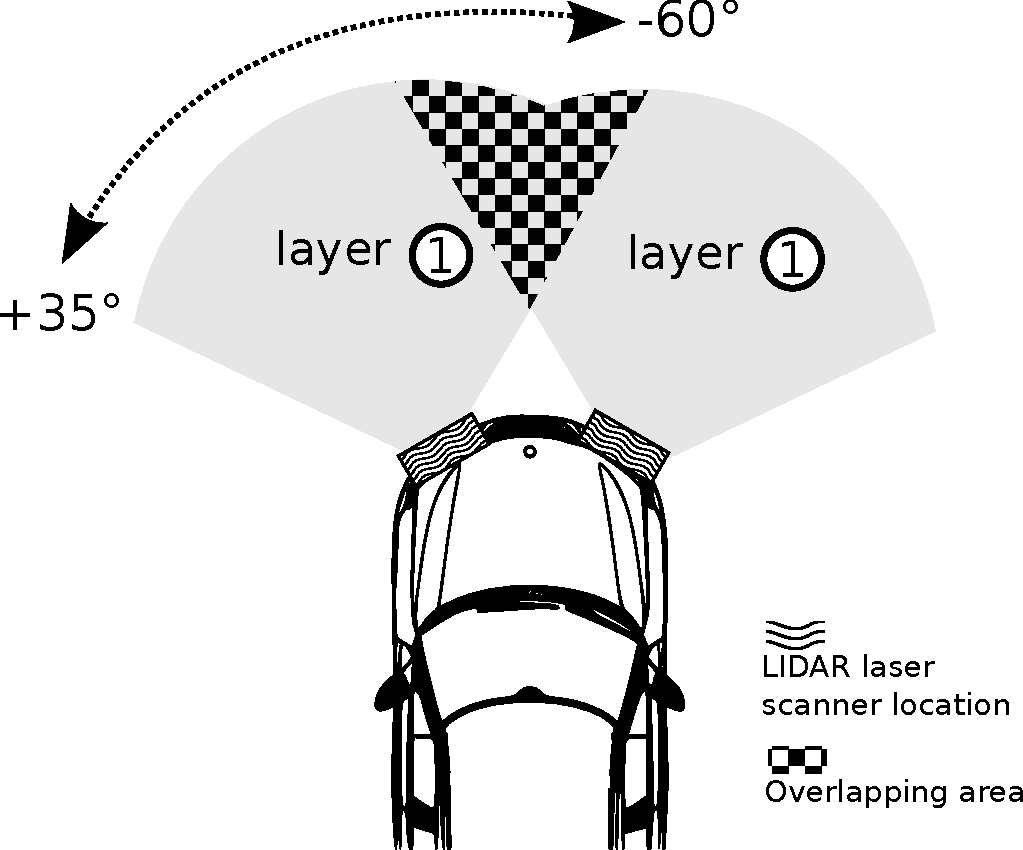
\includegraphics[scale=0.3]{../img/fig:demonstrator:superior:overlap}
		  \end{figure}   
		  \end{column}
		 \end{columns} 	
	
	\end{frame}

	

	\begin{frame}
		\frametitle{Input preparation}
		\begin{figure}[h]
			\center
			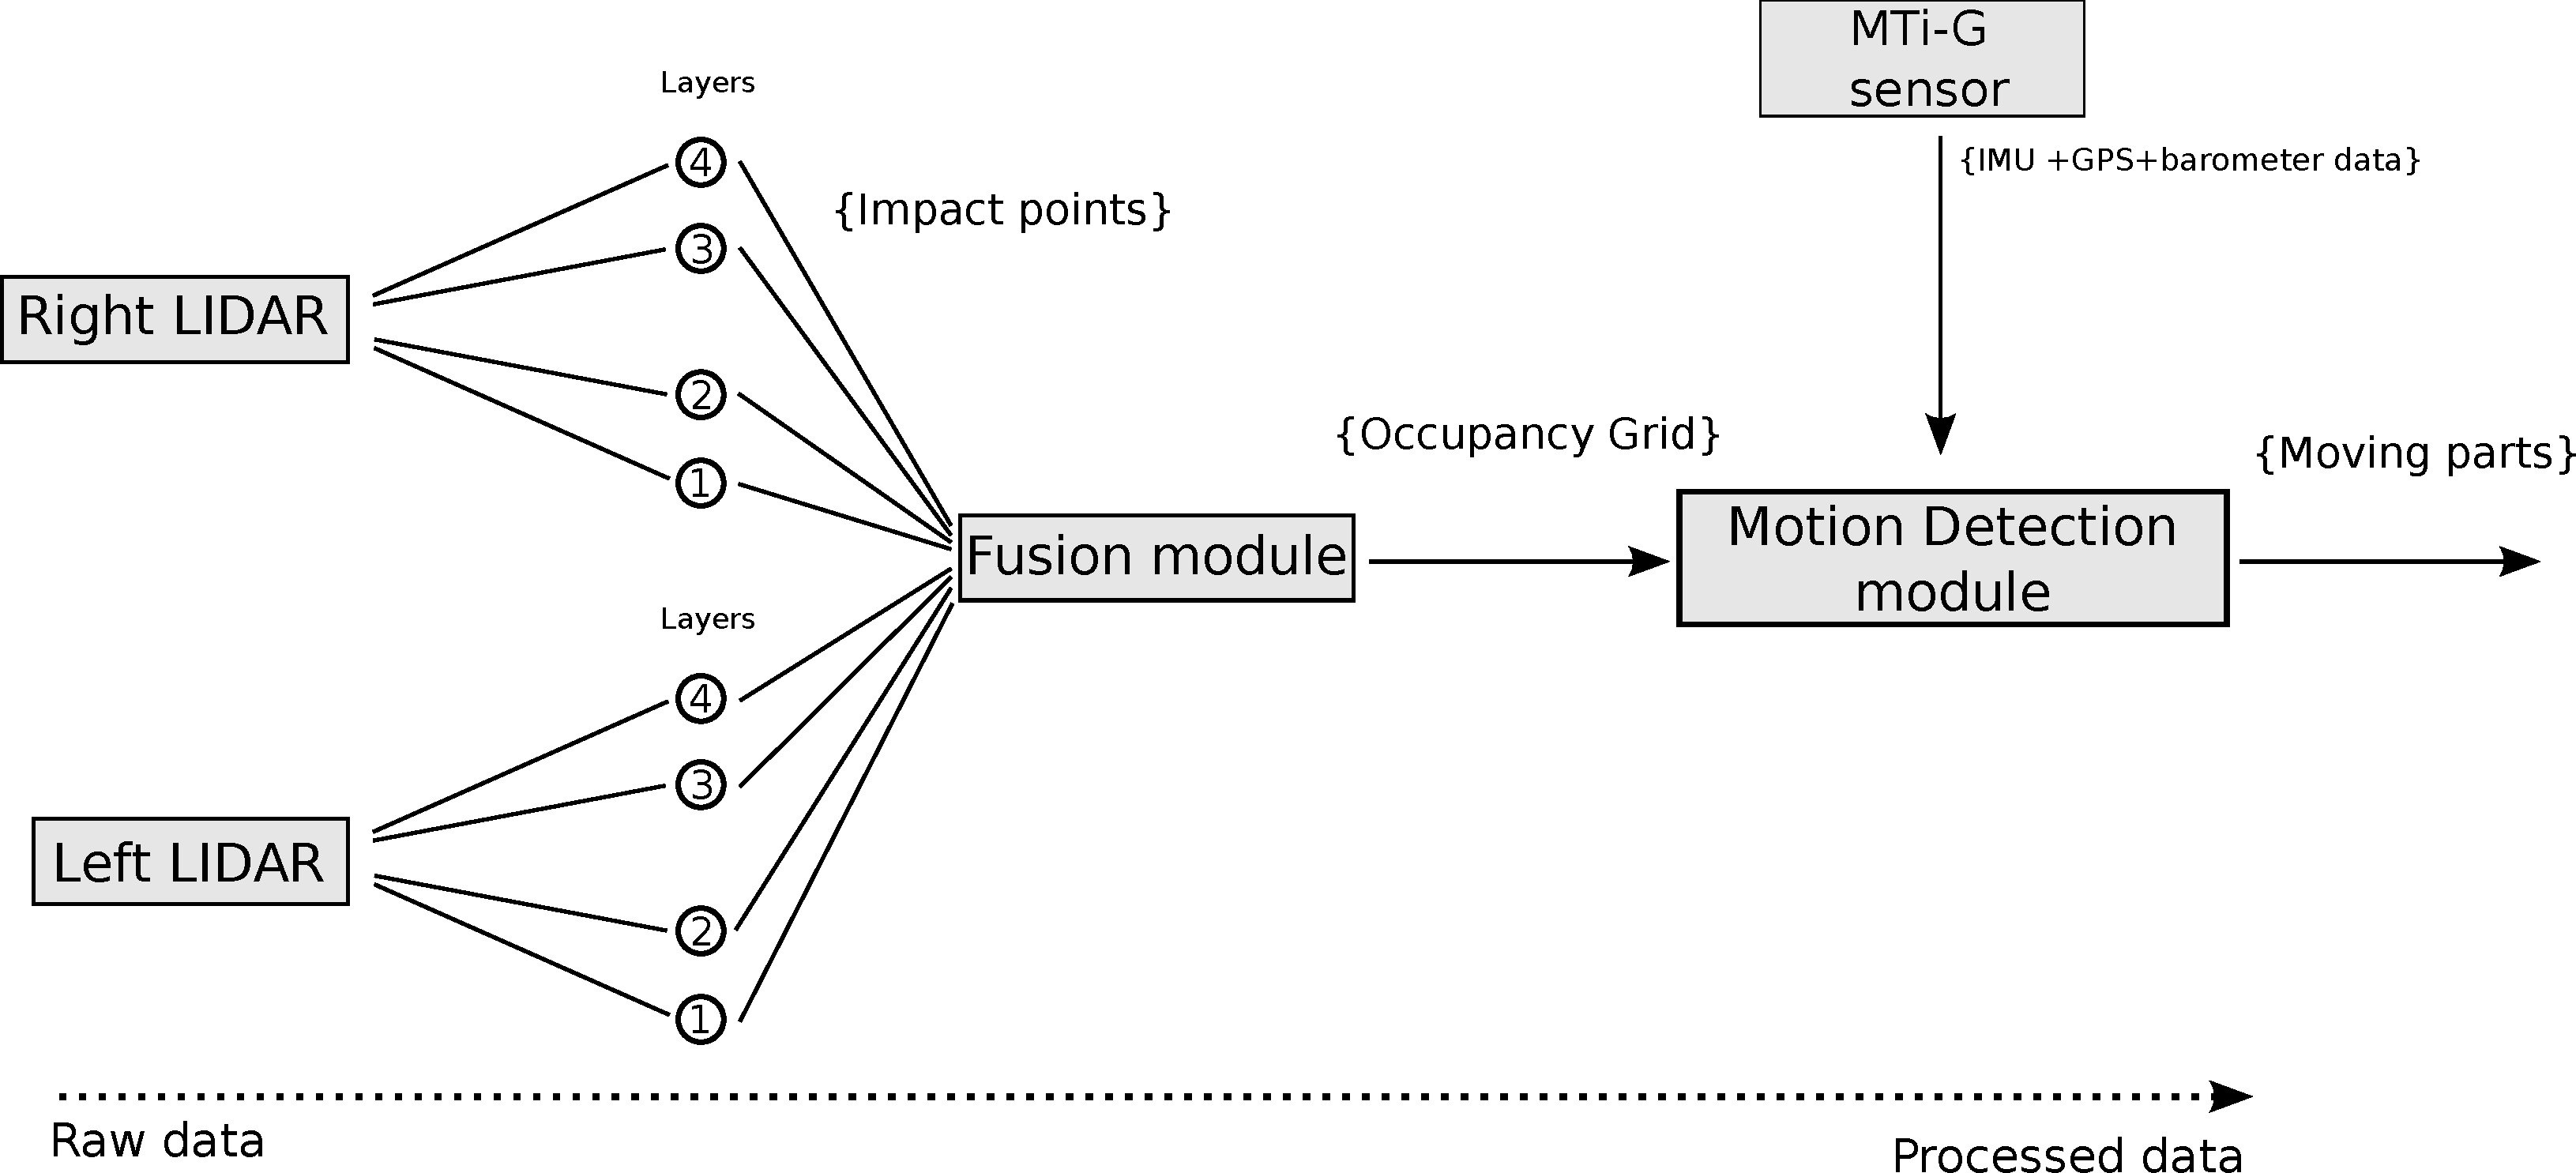
\includegraphics[scale=0.18]{../img/fig:motion:framework}
		\end{figure}
		
		*Linear Opinion Pools \cite{ADARVE-2012-671211}
	
	\end{frame}

	\begin{frame}
		\frametitle{Input preparation}
		\begin{figure}[h]
			\center
			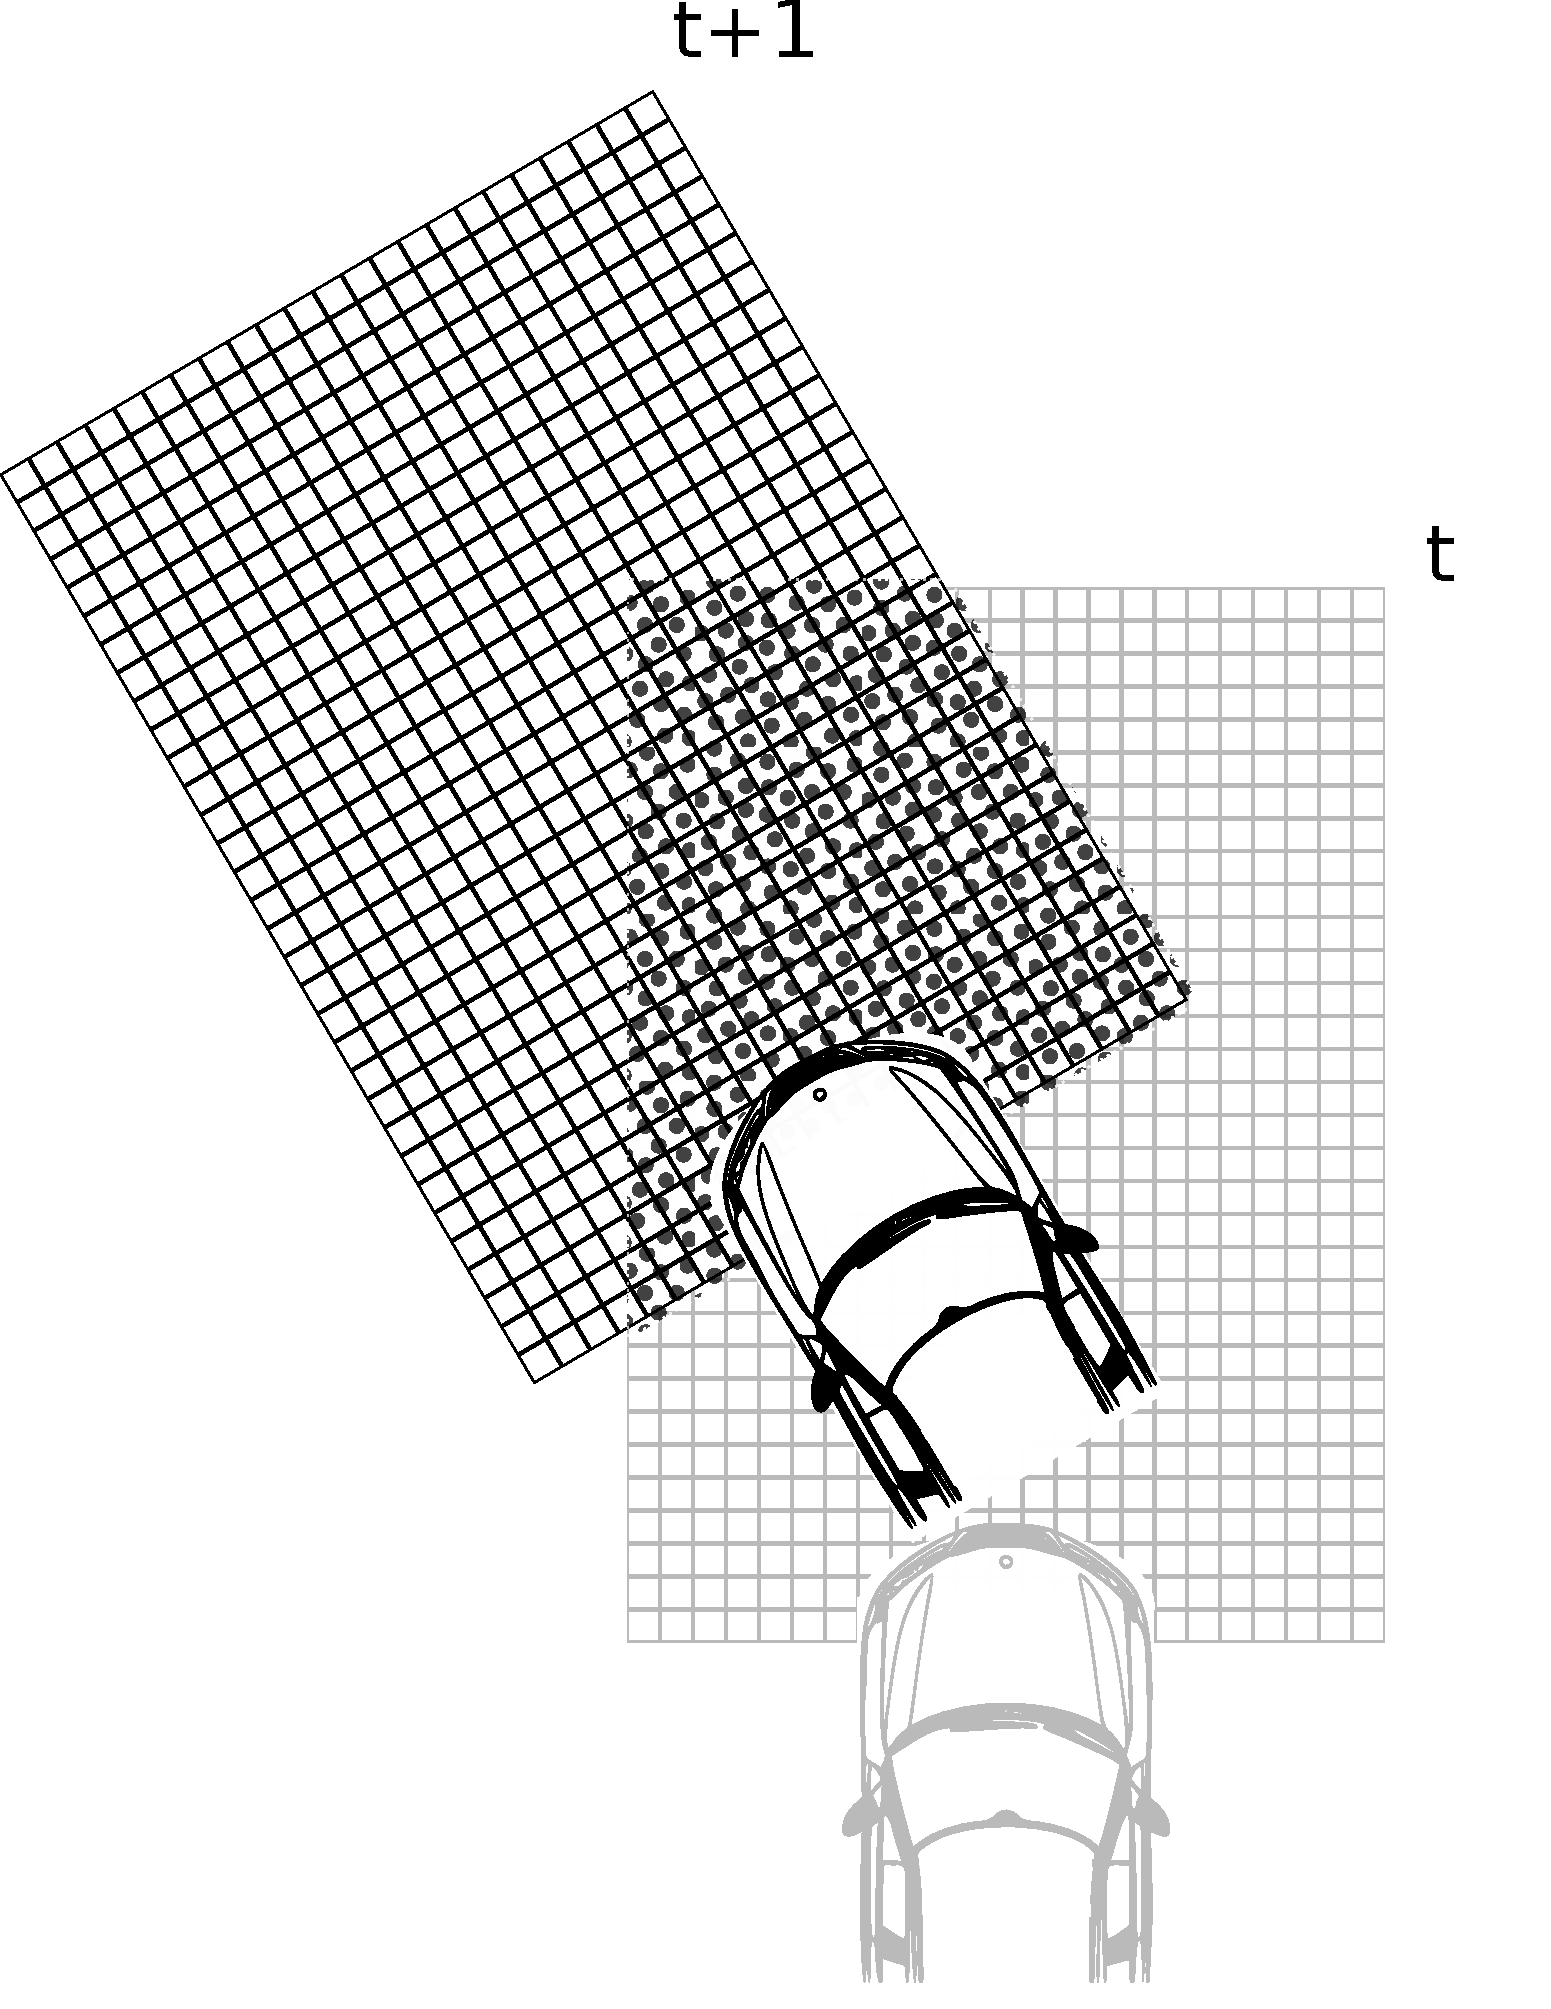
\includegraphics[scale=0.2]{../img/fig:motion:algorithm:nonstatic:01}
		\end{figure}
	
	\end{frame}


	\begin{frame}
		\frametitle{Solution overview}
		\begin{figure}[h]
			\center
			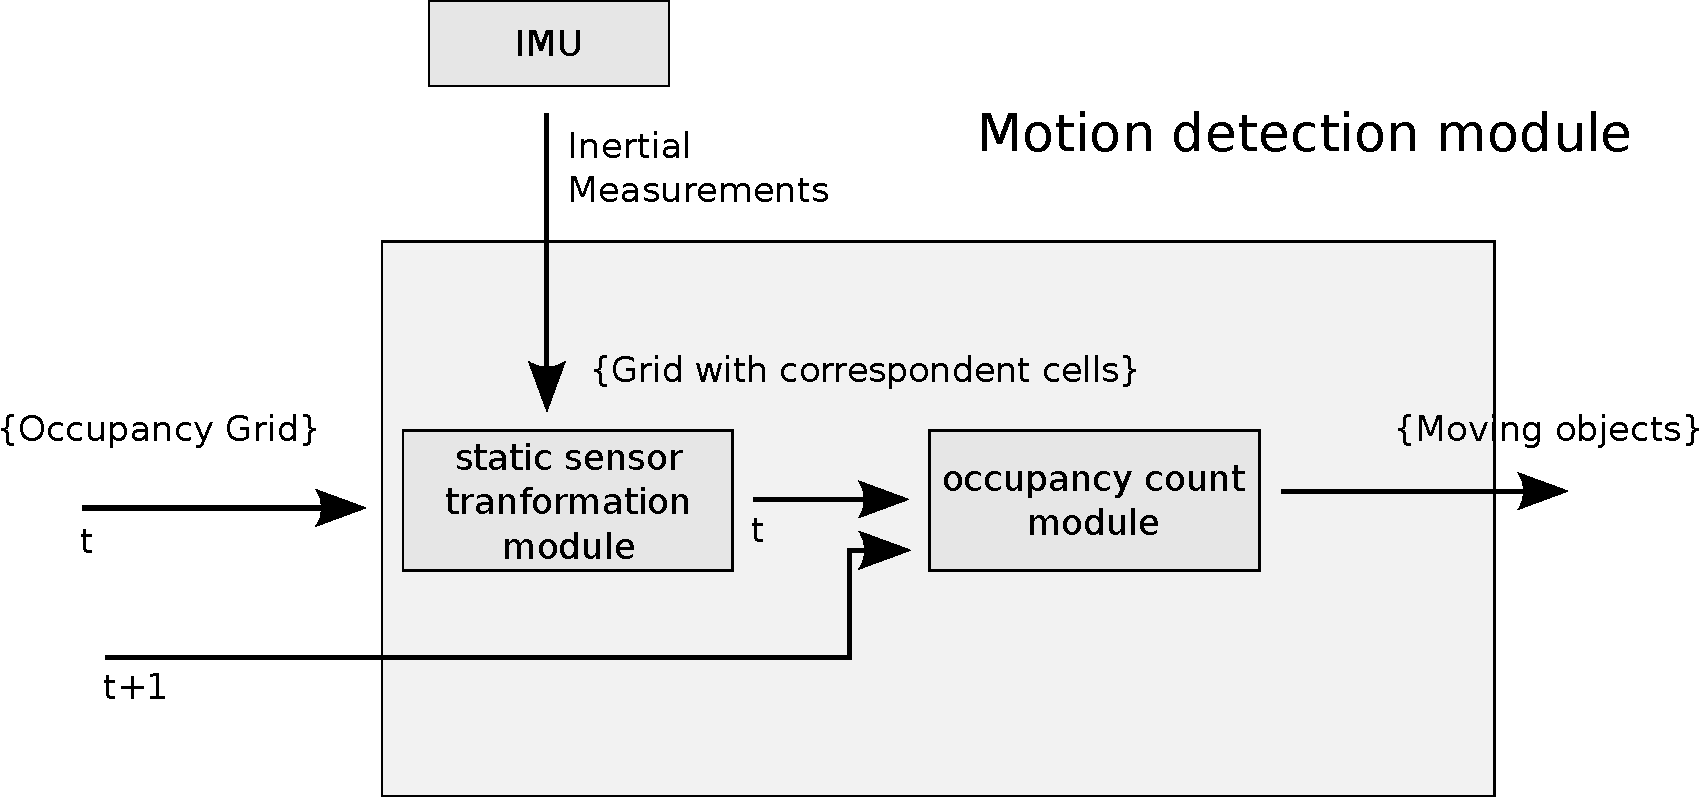
\includegraphics[scale=0.30]{../img/fig:motion:framework:motionmodule}
		 \end{figure}
		
	\end{frame}		
	

\subsection{algorithm}

%%%%%%%%%%%%%%%%%%%%%%%%%%%%%

\section{Experiments}

	\begin{frame}
		\frametitle{Use cases}
		4 use cases were chosen to assess our algorithm:
		\begin{itemize}
		\item Vehicles in urban area
		\item Vehicles in motorway
		\item Vehicle in roundabout
		\item Vehicle in static scenario
		\end{itemize}						
	\end{frame}

\section{Results}

	\begin{frame}
		\frametitle{Vehicles in urban area}
		
		\begin{columns}[t]
			\begin{column}[t]{5cm}
				\begin{exampleblock}{Positive}
				\begin{itemize}
				\item Visibility
				\end{itemize}
				\end{exampleblock}
				\begin{block}{Reason?}
				Bad rotation velocity data (IMU)
				\end{block}
			\end{column}
			\begin{column}[t]{5cm}
				\begin{figure}[h]
				\center
				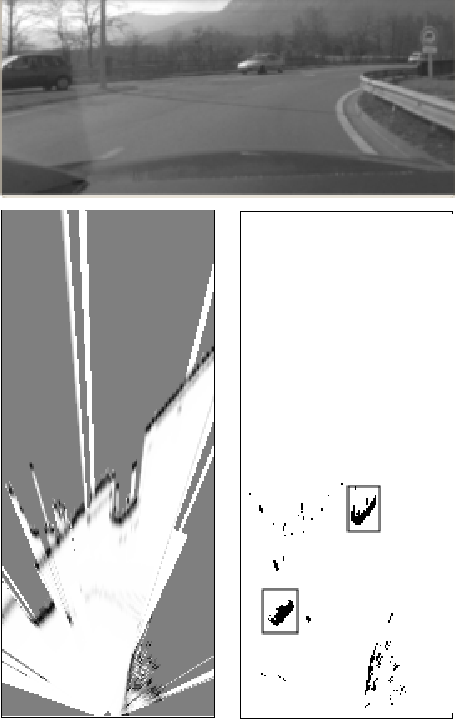
\includegraphics[scale=0.55]{../img/fig:result:scenetwocars}
				\end{figure}
			\end{column}
		\end{columns}		

	\end{frame}
	\begin{frame}
		\frametitle{Vehicles in motorway}
		\begin{columns}[t]
			\begin{column}[t]{5cm}
				\begin{exampleblock}{Positive}
				\begin{itemize}
				\item Good results at high speed (when its most needed)
				\end{itemize}
				\end{exampleblock}
			\end{column}
			\begin{column}[t]{5cm}
				\begin{figure}[h]
				\center
				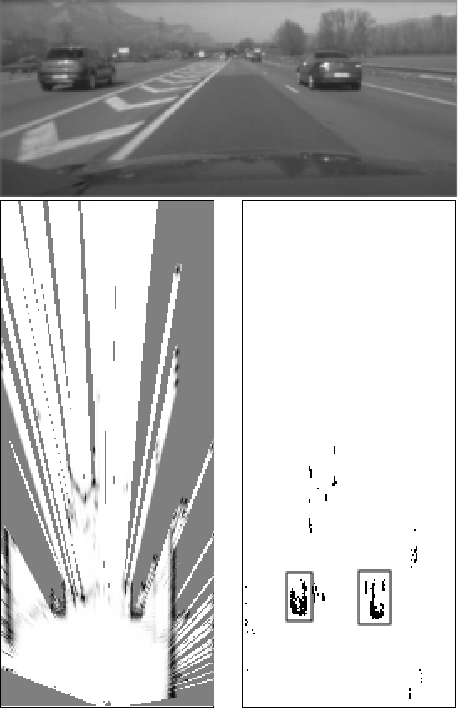
\includegraphics[scale=0.55]{../img/fig:result:scenetwocarshighway}
				\end{figure}
			\end{column}
		\end{columns}		

	\end{frame}
	
	\begin{frame}
		\frametitle{Vehicle in roundabout}
		\begin{columns}[t]
			\begin{column}[t]{5cm}
				\begin{exampleblock}{Positive}
				\begin{itemize}
				\item Very dense pixels
				\end{itemize}
				\end{exampleblock}
			\end{column}
			\begin{column}[t]{5cm}
				\begin{figure}[h]
				\center
				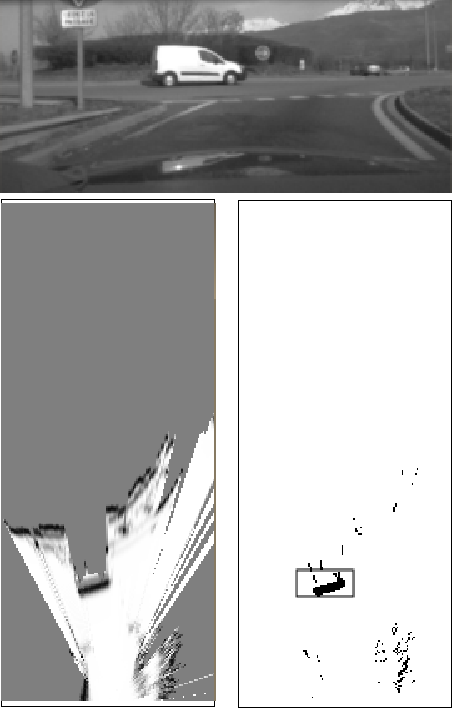
\includegraphics[scale=0.55]{../img/fig:result:scenetwocarrondepoint}
				\end{figure}
			\end{column}
		\end{columns}
	\end{frame}
	\begin{frame}
		\frametitle{Vehicle in static scenario}
		
		\begin{columns}[t]
			\begin{column}[t]{5cm}
				\begin{exampleblock}{Positive}
				\begin{itemize}
				\item Only few sparse pixels
				\end{itemize}
				\end{exampleblock}		
			\end{column}
			\begin{column}[t]{5cm}
				\begin{figure}[h]
				\center
				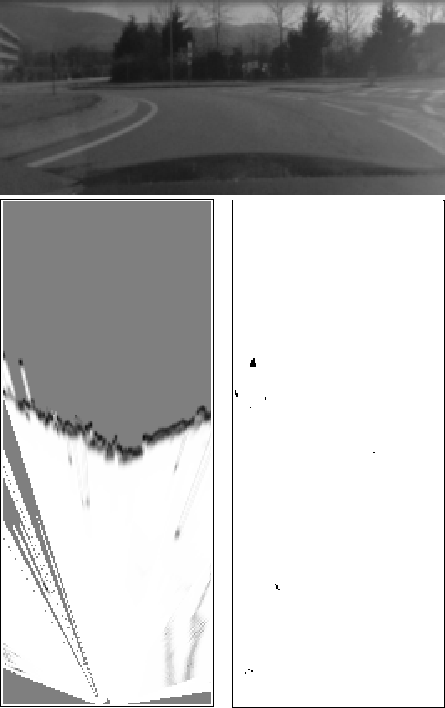
\includegraphics[scale=0.55]{../img/fig:result:scenestatic}
				\end{figure}
			\end{column}
		\end{columns}
	\end{frame}			

	\begin{frame}
		\frametitle{Run time}

		\begin{alertblock}{Performance}
			Run in approximately 3.0ms in a 2.67Mhz processor
		\end{alertblock}		
		
		\begin{exampleblock}{Bright side}
			Still place for optimization
		\end{exampleblock}				
		
	\end{frame}	

	\begin{frame}
		\frametitle{Conclusion}
		
		\begin{block}{Benefits}
			\begin{itemize}
			\item easy to integrate with existing solutions
			\item faster way to classify
			\item still place for improvement
			\end{itemize}
		\end{block}		
		
		\begin{block}{Future work}
			\begin{itemize}
			\item Filtered after all to reduce the noise
			\item Solve the IMU data precision dependency
			\end{itemize}
		\end{block}
		
	\end{frame}

%\begin{thebibliography}{9}
%	\begin{frame}{References}
%		\bibitem{iyengar1991autonomous}
%			Iyengar, S.S. and Elfes, A.
%			\emph{Autonomous Mobile Robots: Control, planning, and architecture}.
%			1991.
%			
%		\bibitem{DBLP:journals/inffus/VuBA11}
%			Trung-Dung Vu, Julien Burlet, Olivier Aycard
%			\emph{Grid-based localization and local mapping with moving object
%              detection and tracking}.
%			2011.			
%
%		\bibitem{hal-00671211}
%			Adarve, Juan David and Perrollaz, Mathias and Makris, Alexandros and Laugier, Christian
%			\emph{Computing Occupancy Grids from Multiple Sensors using Linear Opinion Pools}.
%			2012.
%
% 	\end{frame}
%	\end{thebibliography}

	\begin{frame}{That is it..}
	\begin{alertblock}{}
		\center
		Questions?
	\end{alertblock}
	\end{frame} 	
 	
\bibliographystyle{apalike}
%abbrvnat
%alpha

\bibliography{../report}{} 	

\end{document}